\documentclass[12pt]{report}

% Preamble: Packages and custom settings
\usepackage{amsmath}        % Math environments
\usepackage{amsfonts}       % Math fonts
\usepackage{amssymb}        % Math symbols
\usepackage{graphicx}       % For including images
\usepackage{hyperref}       % For clickable links and cross-references
\usepackage{enumitem}       % Customized lists
\usepackage{geometry}       % Control page margins
\usepackage{fancyhdr}       % Customize headers and footers
\usepackage{xcolor}         % Color text, if needed
\usepackage{pgfplots}       % For plots
\pgfplotsset{compat=1.18}   % Set compatibility to 1.18
\usepackage{circuitikz}     % For circuits!
\usepackage{booktabs}       % Improved tables
\usepackage{siunitx}        % SI units
\usepackage{setspace}       % Custom line spacing
\usepackage{appendix}       % Appendices
% \usepackage{pythontex}      % For Python code
\usepackage{commath}        % For derivatives
\usepackage{cancel}         % Cancel terms in equations
\usepackage{mathtools}      % Extra math tools
\usepackage{titlesec}       % Modern section titles
\usepackage{bookmark}       % Improved bookmarks for navigation
\usepackage{float}          % Improved figure placement
\usepackage{mdframed}       % Framed text blocks

% Custom commands and settings
\sisetup{per-mode = symbol}
\onehalfspacing%
\geometry{margin=2cm,a4paper}
\fancypagestyle{plain}{%
  \fancyhf{}%
  \fancyhead[L]{\textbf{Nicholas Russell}}%
  \fancyhead[C]{\textit{ELECTENG 332 Notes}}%
  \fancyhead[R]{August 10th, 2024}%
  \fancyfoot[C]{\thepage}%
  \renewcommand{\headrulewidth}{0.4pt}%
  \renewcommand{\footrulewidth}{0pt}%
}

\setlength{\headheight}{16.5pt}

% Custom section titles
\titleformat{\chapter}[display]
  {\normalfont\LARGE\bfseries}{\chaptertitlename\ \thechapter}{20pt}{\LARGE}
\titleformat{\section}
  {\normalfont\Large\bfseries}{\thesection}{1em}{}
\titlespacing*{\chapter}{0pt}{50pt}{40pt}
\titlespacing*{\section}{0pt}{20pt}{10pt}

% Document information
\title{ELECTENG 332 Notes}
\author{Nicholas Russell}
% \date{August 10th, 2024}

% Document content
\begin{document}

\begin{titlepage}
    \centering
    \includegraphics[width=0.7\textwidth]{DECSE-HC-4C-01.png}\\[1cm] % University Dept. Logo
    % University and Course Information
    {\LARGE \textbf{ELECTENG 332}}\\[0.5cm]
    {\Large Notes on Control Systems}\\[0.5cm]
    % Add a personal touch with a subtitle or quote
    {\textit{Dear god help me, not another one\dots\ }}\\[2cm]
    % Your Name and Date
    {\large by}\\[0.3cm]
    {\large \textbf{Nicholas Russell}}\\[1.4cm]
    {\large August 10th, 2024}
    \vfill % Push the following text to the bottom of the page
    % Department/University Information
    {\large Department of Electrical, Computer, and Software Engineering}\\[0.3cm]
    {\large Faculty of Engineering}\\[0.3cm]
    {\large University of Auckland}
\end{titlepage}

\tableofcontents
\newpage

\chapter{\textcolor{blue}{Module 1: Basics of Signals and Systems}}

\section*{Learning Outcomes}
\begin{enumerate}[label=\blacktriangleright, leftmargin=*, itemsep=0.5em]
    \item Uniqueness of the Exponential Signal
    \item Concept of Engineering Infinity
    \item Concept of Complex Frequency
    \item Classification of Signals: Energy \& Power
    \item Classification of Systems
    \item What is a Control System
    \item Classification of a Control System: Open-loop \& Closed-loop
\end{enumerate}

\section{Topic 1: Importance of Exponential Functions}
The Exponential function, written as either
\(e^{ax}\) or \(e^{at}\) depending on whether it is \(f(t)\) or \(f(x)\),
has properties that make it mathematically unique.

\begin{enumerate}
    \item The derivative (rate of change) of the exponential function is the exponential function itself. More generally, this is a function whose rate of change is proportional to the function itself.
          \[
              \od{e^{ax}}{x} = ae^{ax}
          \]
    \item The integral of the exponential function is also the exponential function itself.
          \[
              \int e^{ax} \dif x = \frac{1}{a}e^{ax}
          \]
\end{enumerate}

\section{Topic 2: Concept of Engineering Infinity}
Consider a signal \(e^{-at}\). The time constant for this signal is \(T = \frac{1}{a}\). Theoretically, the signal is meant to decay to zero as time approaches infinity, i.e.
\[ 
    \lim_{t \to \infty} e^{-at} = 0 
\] 
But in practice, this is not the case, as its value will be very, very small after five time constants \(5T\). This is the \emph{Concept of Engineering Infinity}.

\section{Topic 3: Concept of Complex Frequency}
Complex frequency is found commonly in electrical engineering. It is often notated as \( j\omega \) or \( s = \sigma \pm j \omega \). These frequencies always come in pairs, so the use of \( \pm \) is implicit to this, as complex numbers have complex conjugates, i.e.
\(s = \sigma + j \omega \) has the conjugate \(s = \sigma - j\omega \).

\begin{figure}[H]
    \centering
    \usetikzlibrary{arrows.meta}
    \begin{tikzpicture}
        \begin{axis}[
                axis equal,
                axis x line = middle,
                axis y line = middle,
                xmin=-2, xmax=2,
                ymin=-2, ymax=2,
                xlabel={Re(z)},
                ylabel={Im(z)},
                grid=major,
                enlargelimits=true,
            ]
            % Plot the circle |z| = sqrt(2)
            \addplot[domain=0:360, samples=200, smooth, very thick]({sqrt(2)*cos(x)}, {sqrt(2)*sin(x)});
            \addplot[only marks, mark=*, red, mark size=2pt] coordinates {%
                    (1,1) (-1,1) (1,-1) (-1,-1)
                };
            % Draw vectors from origin to each point
            \addplot[->, black, very thick, >= latex] coordinates {(0,0) (1,1)};
            \addplot[->, black, very thick, >= latex] coordinates {(0,0) (-1,1)};
            \addplot[->, black, very thick, >= latex] coordinates {(0,0) (1,-1)};
            \addplot[->, black, very thick, >= latex] coordinates {(0,0) (-1,-1)};
        \end{axis}
    \end{tikzpicture}
    \caption{Plot of the circle \(|z| = \sqrt{2}\)}\label{fig:pgfplots-complex-plane-1}
\end{figure}

\noindent This is also backed up by De Moivre's Formula, which is defined mathematically as:
\begin{gather*}
    \forall x \in \mathbb{R}, \quad \forall n \in \mathbb{Z}, \\
    e^{j n x} = \cos(n x) + j \sin(n x)
\end{gather*}
Or more generally for our applications:
\begin{gather*}
    e^{jx} = \cos(x) + j\sin(x) \\
    \text{Where} \, x \in \mathbb{R}\, \text{(\(x\) is Real)} \\
    \text{and} \, j \equiv i = \sqrt{-1}.
\end{gather*}
\newpage
\noindent This means that:
\begin{figure}[H]
    \centering
    \begin{mdframed}
        \begin{center}
            \textcolor{red}{\emph{A complex frequency \(j\omega \) represents a pure sinusoidal signal of frequency \(\omega \) \unit{\radian\per\second}}}
        \end{center}
    \end{mdframed}\label{fig:complex-sinusoid-def-1}
\end{figure}
\noindent For example, if a signal has a complex frequency  \complexqty[output-complex-root=j, complex-root-position=before-number]{314i}{\radian\per\sec}, then this corresponds to a pure sinusoid of frequency \SI{314}{\radian\per\sec} (i.e. \SI{50}{\hertz}). Furthermore:
\begin{figure}[H]
    \centering
    \begin{mdframed}
        \begin{center}
            \textcolor{red}{%
                \emph{A complex frequency \(s = \sigma + j\omega \) represents an exponentially
                    damped signal of frequency \(\omega \) \unit{\radian\per\second}, and decays/amplifies at a rate decided by \(\sigma \).}}
        \end{center}
    \end{mdframed}\label{fig:exp-damped-sinusoid-def-1}
\end{figure}
\noindent For example, the signal \( e^{- 10t}\sin(40\pi t) \) would look like this:
\begin{figure}[H]
    \centering
    \begin{tikzpicture}
        \begin{axis}[
                domain=0:1, % Domain for the variable t
                samples=1000, % Number of samples to plot (higher for smoother curve)
                xlabel={$t$},
                ylabel={$e^{-10t} \sin(40\pi t)$},
                grid=major,
                thick,
                enlargelimits=true,
                axis y line = center,
                axis x line = left,
                ymin=-1, ymax=1,
                xmin=0, xmax=1,
                ytick={-1,-0.8,-0.6,-0.4,-0.2,0,0.2,0.4,0.6,0.8,1},
            ]
            % Plot the function e^{-10t} * sin(40*pi*t)
            \addplot[blue, thick] {exp(-10*x) * sin(deg(40*pi*x))};
        \end{axis}
    \end{tikzpicture}
    \caption{Plot of the signal \(e^{-10t}\sin(40\pi t)\).}\label{fig:exp-damped-sinusoid-plot-1}
\end{figure}

\section{Topic 4: What are Signals?}

\clearpage

\chapter{\textcolor{blue}{Module 2: Mathematical Modelling of Dynamic Systems}}

\section{Topic 1: [Topic Name]}

\section{Topic 2: [Another Topic Name]}

\clearpage

\chapter{\textcolor{blue}{Module 3: Concept of Block Diagram Representation \& Characteristics of Feedback Systems}}

\clearpage

\chapter{\textcolor{blue}{Module 4: Time Domain Analysis of Linear Systems}}
% \zeta cannot be greater than 1, less than 0. 
% (for some reason \zeta is typeset as \xi in notes, unsure if typo)
\clearpage

\chapter{\textcolor{blue}{Stability Analysis of Linear Systems}}
% poles must not be in right hand side of plane, if true, system unstable.

\end{document}
